\documentclass[
 a4paper,twocolumn,showpacs,aip,groupedaddress,%
  eqsecnum,notitlepage,showkeys,cha,longbibliography,10pt
]{revtex4-1}
\usepackage[english]{babel}
\usepackage[utf8x]{inputenc}
\usepackage[T1]{fontenc}
\usepackage{amssymb}
\usepackage{amsmath,latexsym}
\usepackage{graphicx}
\usepackage{dcolumn}
\usepackage{tikz}
\usepackage{natbib}
\usepackage{float}
\usepackage[hyperref]{}
\usepackage[export]{adjustbox}


\usepackage[a4paper,top=1.8cm,bottom=1.8cm,left=1.5cm,right=1.5cm]{geometry}
\usepackage[skip=5pt, font=scriptsize, labelfont=bf, justification=raggedright]{caption}

\usepackage{titlesec}

\titlespacing\section{0pt}{12pt plus 4pt minus 2pt}{0pt plus 2pt minus 2pt}

\graphicspath{ {Images/} }

\begin{document}

\title{\LARGE{Fabrication and Measurement of a Niobium SQUID}}

\author{Lindsey Keary}
\affiliation{ 
Student Number : 17099595, l.keary.17@ucl.ac.uk, University College London
}
\date{\today}

\begin{footnotesize}
\begin{abstract}
The process of fabricating a direct current (dc) superconducting quantum interference device (SQUID) on a pre-patterned silicone ($Si$) wafer with a niobium ($Nb$) film is described. The area of the loop is $9 \times {10^{ - 12}}$ m. The length of the left and right parallel Dayem junctions are approximately 80 nm and 50 nm, respectively. The width of junctions are approximately 70 nm and 50 nm for the left and right junctions, respectively. The critical temperature $T_C$$ = ($8.89 $\pm$ 0.01) of $Nb$ is measured during cryostat cooling of the sample in liquid helium ($He$). The current-voltage (I-V) characteristic plot for the SQUID exhibits hysteric features with the recorded critical current of $I_C$=(5.31 $\pm$0.05) $\mu$A in a magnetic field $B\approx$=0. Investigating the oscillations of the $I_C$ as a function of $B$ requires further measurements to determine the reproducibility an apparent oscillation with a period of 2 mT when $B$ is increased from 0 to 5 mT. 
\end{abstract}
\end{footnotesize}

\maketitle

% \begin{quotation}
The ``lead paragraph'' is encapsulated with the \LaTeX\ 
\verb+quotation+ environment and is formatted as a single paragraph before the first section heading. 
(The \verb+quotation+ environment reverts to its usual meaning after the first sectioning command.) 
Note that numbered references are allowed in the lead paragraph.
%
The lead paragraph will only be found in an article being prepared for the journal \textit{Chaos}.
\end{quotation}
\begin{footnotesize}
\section{\label{sec:level1}Introduction}
In recent years the miniaturisation, to micro and nano-chip scales, has been the focus for development of various quantum sensing devices. SQUIDs are devices which enable high precision measurement of small changes in the magnetic flux due to period oscillations of the critical current, $I_C$ in an applied magnetic flux, $\Phi$ $^[$\citep{Podd2007Micro-SQUIDsJunctions}${}^]$. Developing devices which can measure the magnetisation of particles of the order of nanometers has applications in a range of fields including biomedicine, telecommunication and quantum computing $^[$\citep{Hao2015FabricationJunctions}${}^]$.

Typical fabrication techniques produce a dc nanoSQUID consisting of two parallel Dayem Josephson junctions (JJs) connected to a superconducting loop $^[$\citep{Hao2015FabricationJunctions}${}^]$. These quantum sensing devices exploit the Josephson effect and flux quantisation. At temperatures below $T_C$ for superconducting, Josephson tunneling of Cooper pairs through the junction between two superconductors creates a supper current $I_S=I_0\sin\delta$. The phase difference between the superconducting materials is $\delta$. For Type 1 superconductors below $T_C$ the magnetic flux in the loop is expelled. However, in the case of a Type 2 superconductor such as $Nb$ vortices of magnetic flux can penetrate through in quantised units of the flux quantum ${\Phi _0}$=h/2e $^[$\citep{Clarke2005TheHandbook}${}^]$.
\section{\label{sec:level1}Fabrication}
To observe typical characteristics of a SQUID such as the sinusoidal current-phase relationship (CPR), the niobium coherence length of $\xi$=40 nm  $^[$\citep{Clarke2005TheHandbook}${}^]$ must be approximately equal to the Dayem bridge dimensions $^[$\citep{Hao2015FabricationJunctions}${}^]$. In addition, the effective area of the superconducting ring is $^[$\citep{Troeman2007NanoSQUIDsConstrictions}${}^]$
\begin{equation}
\label{eq:effectivearea}
{A_{eff}} = {\Phi _0}/{B_0}
\end{equation}
where one period of the voltage-magnetic field (V-B) oscillation requires a magnetic field strength of ${B_0}$. The approximate value of $B_0$ for this fabricated SQUID is 2 mT.  

\begin{figure}[b]
\centering
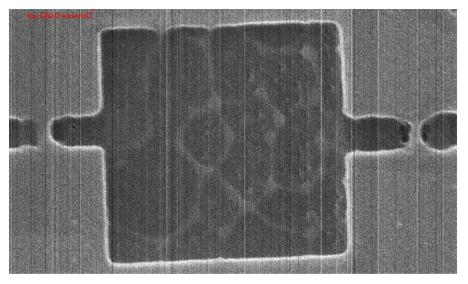
\includegraphics[width=0.4\textwidth]{B3after}
\caption{\label{fig:B3after}Fabricated SQUID on $Nb/Si$ chip. The loop is $\approx0.91\times {10^{ - 12}}$ m.The length ($l$) and width ($w$) of the left and right Dayem junctions are ($l$$\approx$ 80 nm, $w\approx$ 70 nm), ($l\approx$ 50 nm, $w$$\approx$ 50 nm), respectively.}
\end{figure}

The 50 nm thick $Nb$ film is coated on a 100 mm $Si$ wafer. Prior preliminary fabrication has been completed to produce a patterned chip the with electrical contact pads using polymethyl methacrylate (PMMA) resist and electron beam lithography (EBL) $^[$\citep{Granata2008AnApplications}${}^]$. The SQUID is created within the patterned section of the $Nb/Si$ chip by milling portions of the $Nb$ using a neon ($Ne$) focused ion beam (FIB). When the extraction field is applied the $Ne$ ions collect in approximately 10 nm cone at the point of the FIB needle $^[$\citep{Giannuzzi1999AScienceDirect_com}${}^]$. 

An acceleration voltage of $\approx$ 25 keV is used to fire the ions towards the sample. Sputtered particles referred to the injection of $Ne$ particles into the $Nb$ material when completing FIB milling
$^[$\citep{Giannuzzi1999AScienceDirect_com}${}^]$ and the FIB has Gaussian beam profile with a beam waist of $\approx$30 nm $^[$\citep{Troeman2007NanoSQUIDsConstrictions}${}^]$. Therefore there is an uncertainty associated with milling the $A_{eff}$ of the SQUID loop and the dimensions of the JJs. The detection of secondary electrons produced by the FIB enables image construction of the SQUID as shown in Fig.(\ref{fig:B3after}). The length ($l$) and width ($w$) of the left and right Dayem junctions are ($l$$\approx$ 80 nm, $w$$\approx$ 70 nm), ($l\approx$ 50 nm, $w$$\approx$ 50 nm), respectively. When the $l\ge3\xi$ the single-valued sinusoidal CPR is lost $^[$\citep{Troeman2007NanoSQUIDsConstrictions}${}^]$. The square superconducting loop has an $A_{eff}\approx0.91\times {10^{ - 12}}$ m. The sensitivity of the SQUID device is a function of the loop $A_{eff}$ $^[$\citep{Granata2008AnApplications}${}^]$.

\section{\label{sec:level1}Measurement}

\begin{figure}[b]
\centering
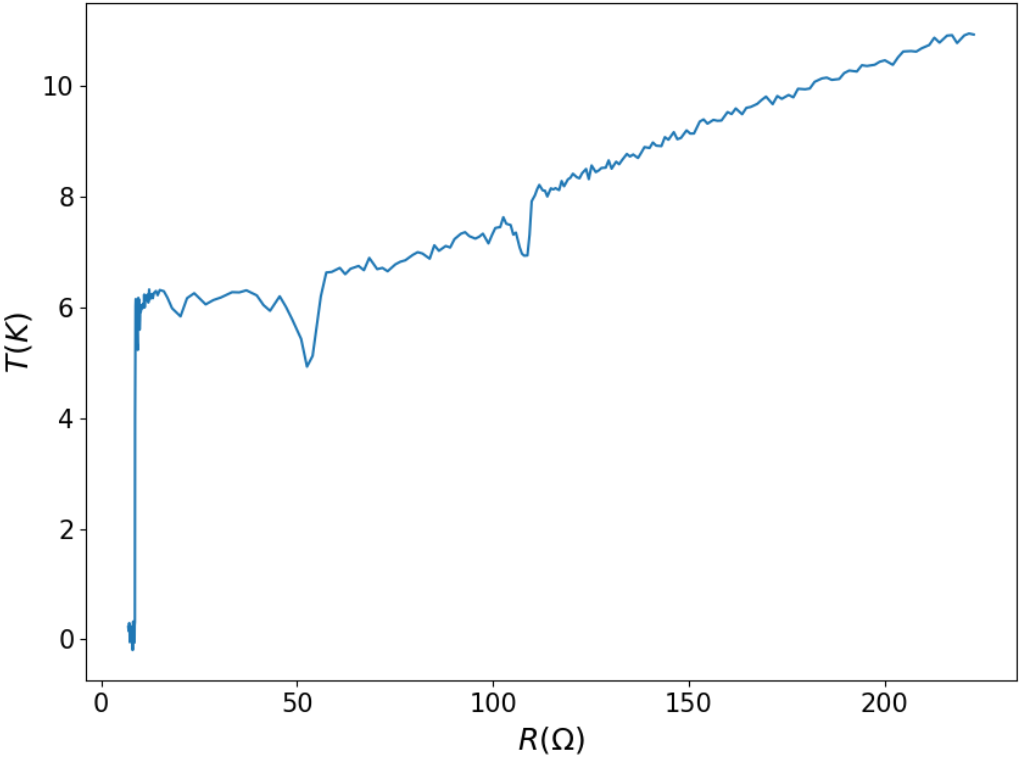
\includegraphics[height=0.275\textwidth,keepaspectratio]{RTPlot}
\caption{\label{fig:RTPlot}R-T plot for niobium where $T_C$$ = ($8.89 $\pm$ 0.01) K.}
\end{figure}

The SQUID electrical contact pads are wire bonded to a printed circuit board (PCB) in a four point connection. The combined sample is mounted within the inner vacuum chamber (IVC) of the cryostat where cooling processes using liquid ${}^4He$ reduces the sample temperature. Firstly the IVC is initially evacuated before a small amount of ${}^4He$ exchange gas enters the IVC by flushing the needle value and 1k pot valve to produce a $\approx$ 5 mbar pressure. Heat exchange with the 1 K pot reduces the temperature of the sample to $T_S$ $\approx$ 5 K. The thermal contact of the IVC and 1 K pot is removed. To achieve temperature cooling of $T_S$ $\approx$ 300 mK, ${}^3He$ must be condensation. The 1 K pot reaches a temperature below the boiling point of ${}^3He$, by liquid $^4He$ pumping, $^3He$ in contact with the 1 K pot is condensed $^[$\citep{HeManual}$^]$. Close cycle sorb pumping of $^3He$ through a charcoal sample in thermal contact with IVC is implemented and the sample reaches the base line temperature of $\approx$ 300 mK $^[$\citep{HeManual}$^]$. 

The initial dc measurement is completed during the cooling process by applying a small current source which flows through an uninterrupted section of $Nb$ film between the contact pads. The applied current ranges between $\pm$ 5 $\mu$A and the Voltage is measured.The resistance-temperature (R-T) plot is in Fig.(\ref{fig:RTPlot}) illustrates where the resistance drops to 0 and $Nb$ become superconducting at $T_C$ = (8.89 $\pm$ 0.01) K. The points at which the value of resistance appears to dip occurs when the cryostat probe is being lowered further into the liquid $4^He$ container.

\begin{figure}[t]
\centering
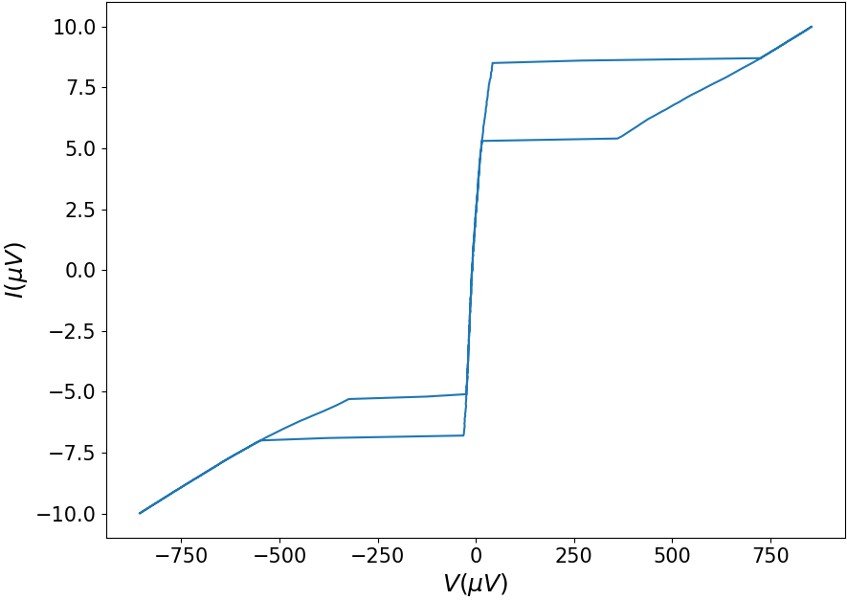
\includegraphics[height=0.275\textwidth,keepaspectratio]{IVplot}
\caption{\label{fig:IVplot}I-V curve for $B$ $\approx$ 0 mT. For positive current values $I_C$=(5.31 $\pm$0.05) $\mu$A, $I_{SW}$=(8.45 $\pm$0.05) $\mu$A. For negative current values $I_C$=-(5.30 $\pm$ 0.05) $\mu$A, $I_{SW}$=-(7.13 $\pm$0.05) $\mu$A}
\end{figure} 

The $I-V$ slope is measured by applying a dc current source to the SQUID in an applied $B$=0 field where $T_S\approx$ 0.3 K. The $I-V$ slope shown in Fig. (\ref{fig:IVplot}) exhibits a hysteric behaviour. This behaviour is expected to occur in weak-link JJs when $T_S$ is below 1.5 K $^[$\citep{Hao2015FabricationJunctions}$^]$. As the current is increased from 0 to 10 $\mu$A, the switching current $I_{SW}$=(8.45 $\pm$0.05) $\mu$A is the point at which the SQUID resistance becomes non-zero. The current source is then decreased to 0 and the critical current $I_C$=(5.31 $\pm$0.05) $\mu$A is observed as $Nb$ returns to being superconducting. The hysteric behaviour is believed to be due to current crowding through the JJs which results in heating of the device. This heating effect generates "hot spots" within the device when the current applied is > $I_{SW}$ $^[$\citep{Podd2007Micro-SQUIDsJunctions}$^]$. The asymmetry of the hysteresis for positive and negative source $I$ is related to the asymmetry of the left and right Dayem junction dimensions. The magnitude of the negative $I_{SW}$ is notably smaller than the positive $I_{SW}$. However the magnitude of $I_C$ does not change when the dc current is negative since $I_C$ is an bulk property of the $Ni$ SQUID.

The $I-V$ slope measurements are repeated throughout magnetic field sweeping of the SQUID in a range of $B$= $\pm$5 mT. For each $I-V$ data set there is 400 points which corresponds to the current increasing from 0 to 10 $\mu$A then decreasing to -10 $\mu$A and finally increasing to 0. The positive and negative $I_C$ values are obtained for each $I-V$ data set. The applied $B$ follows the same sequence of measurement as described for $I-V$ where the increment change in the applied field for each step is 0.04 mT. The temperature of the sample began increasing as the supply of ${}^4He$ ran out so the data for $B$ < 0 is disregarded.

\begin{figure}[b]
\centering
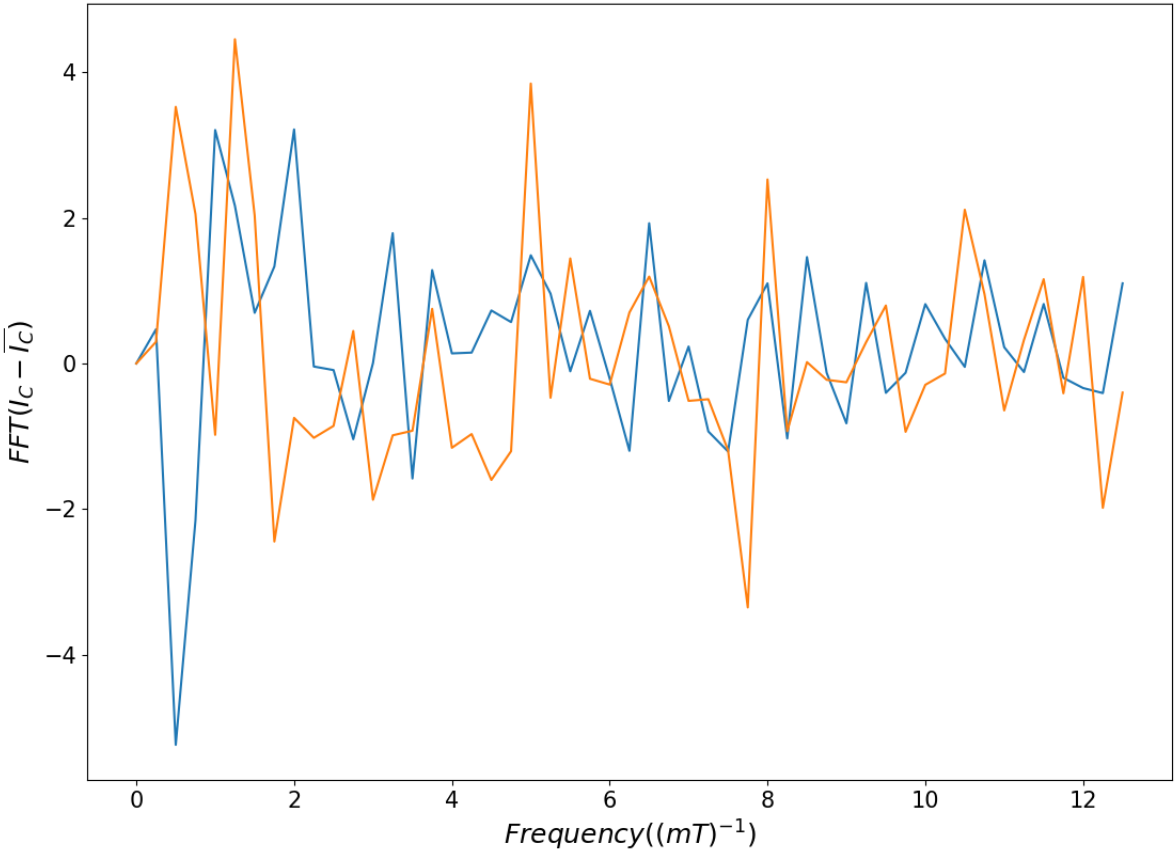
\includegraphics[height=0.275\textwidth,keepaspectratio]{ICbothB}
\caption{\label{fig:ICbothB}The FFT signal of the magnitude of the offset corrected positive (blue line) and negative (orange line) $I_C$ vs. $B$.}
\end{figure}

The range of $B$ is chosen as there is expected to be $\approx$9 periods of $\Phi _0$ for $B$ between 0 and 5 mT. However, there was no discernible periodic motion observed when plotting the positive and negative $I_C$ values against $B$. The Fast Fourier Transform (FFT) is applied to the magnitude of the offset corrected $I_C$ as shown in Fig. (\ref{fig:ICbothB}) when $B$ is increased from 0 to 5 mT. There are many frequency peaks observed in Fig. (\ref{fig:ICbothB}) which is expected to be due to the signal being noisy. However, a large peak is present for positive $I_C$ at a frequency of $\approx$ 0.5 (mT)\textsuperscript{-1}. This period corresponds to the calculated $B_0\approx$ 2 mT using Eq. \ref{eq:effectivearea} where $A_{eff}\approx$ $1 \times {10^{ - 12}}$ m. There is a peak also present at $\approx$ 0.5 (mT)\textsuperscript{-1} for negative $I_C$. However, the peak amplitude is not as large and there are other peaks at different frequency values with a similar amplitude. The FFT signal of the linear fit $R$ is is shown in Fig. (\ref{fig:RvsB}) where a large amplitude peak is also observed at $\approx$ 0.5 (mT)\textsuperscript{-1}. 

The FFT signal of $I_C$ and the FFT signal of linear fit of $R$ for $B$ decreasing towards 0 does not display a significantly large peak at $\approx$ 0.5 (mT)\textsuperscript{-1}. Therefore there is not sufficient evidence that the SQUID is oscillating sinusoidally at a particular frequency.

\begin{figure}[t]
\centering
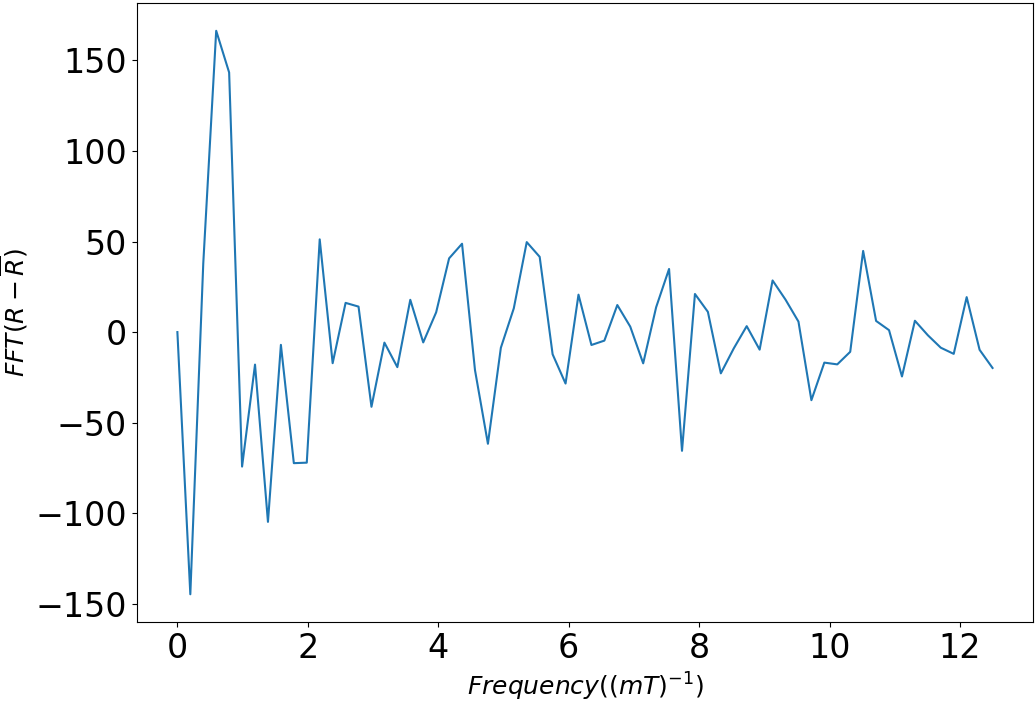
\includegraphics[height=0.275\textwidth,keepaspectratio]{RvsB}
\caption{\label{fig:RvsB}FFT signal of the linear fit resistance vs. $B$.}
\end{figure}


\section{\label{sec:level1}Discussion and Conclusion}
Sinusoidal oscillations of the $I_C$ as a function of the $B$ strength was not observed for this fabricated device. Conversely, there are a number of factors to consider and effects which may be restricting the characteristic SQUID behaviour. Firstly, the JJs dimensions of $l$ and $w$ are greater than the $\xi$ for $Nb$. Although the dimensions do not exceed 3$\xi$, higher harmonic $\sin (N\delta )$ components may be present $^[$\citep{Clarke2005TheHandbook}$^]$. Furthermore, Fig. (\ref{fig:IVplot}) of $I-V$ for the SQUID is hysteric. The production of "hot spots" on the device due to heating effects when  $I\approx$ $I_{SW}$ produces a incoherent CPR $^[$\citep{Podd2007Micro-SQUIDsJunctions}$^]$. Despite observing a large peak at $\approx$ 0.5 (mT)\textsuperscript{-1} for the FFT signal of positive $I_C$ and the linear fit of $R$, these results are not sufficient to verify the sinusoidal relationship between $I_C$ and $\delta$ for an increasing $B$ field. This is due to the absence of a large amplitude peak at $\approx$ 0.5 (mT)\textsuperscript{-1} when the FFT signals are plotted for the $B$ field decreasing from 5 mT to 0. 

In future fabrication and measurement of nanoSQUIDs the dimensions of the bridge should be reduced to as close to $\xi$ as possible without breaking the weak-link JJ. The size of the SQUID loop could be reduced as decreasing the area of the loop increases the device's sensitivity to changes in the magnetic flux. When measuring the $I_C$ oscillations as a function of the applied $B$ field the maximum value of $I-V$ slope should not be hysteric. The hysteric behaviour is expected to be absent for devices where the $I_C$< 25 $\mu$A. Yet for this device $I_C=(5.31 \pm 0.05)$ $\mu$A is measured when $B\approx$0 and the hysteresis is present $^[$\citep{Hao2015FabricationJunctions}$^]$. This may be a result of the low $\approx$ 300 mK temperature of the device so varying the temperature is a possible way to remove the hystersis. Further measurements should be completed over a shortened range of $B$ where more detailed measurements of $I_C$ are required to determine with confidence the observation of magnetic field dependent $I_C$ oscillations.  





\end{footnotesize}


\bibliographystyle{ieeetr}
\tiny
\bibliography{main}

\end{document}